\chapter{Die Benutzeroberfl\"ache}
Dieses Kapitel soll die Konzeption der Oberfl�che begr�nden und deren Nutzung erl�utern.\\

\section{Anforderung}

\section{Auswahl}

\begin{figure} [http]
	
	\centering
	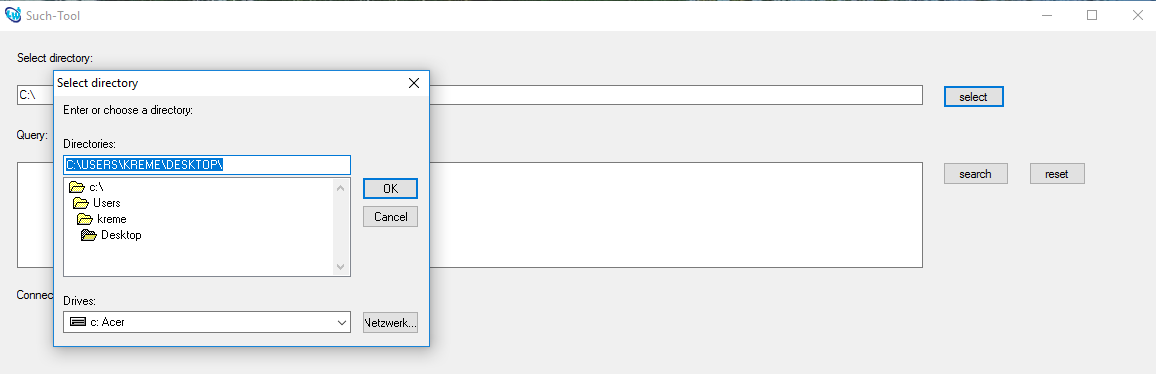
\includegraphics[width=1\textwidth]{images/Select.png}
	\caption{Verzeichnisauswahl (Eigene Abbildung)}
	\label{select}
	
\end{figure}

\section{Suchanfrage}
\begin{figure} [http]
	
	\centering
	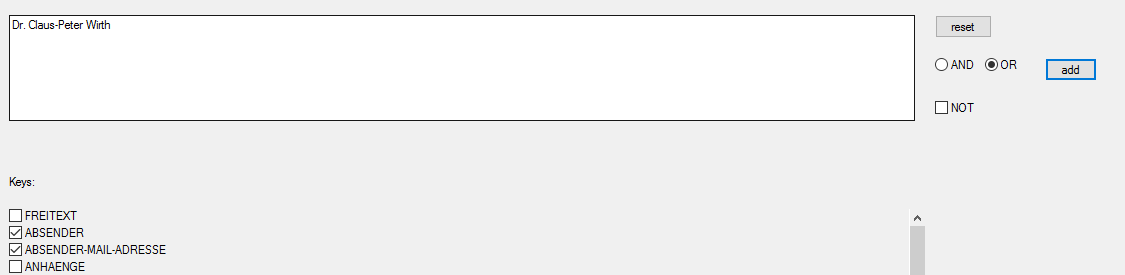
\includegraphics[width=1.1\textwidth]{images/a}
	\caption{Keywords ausw�hlen und intern verkn�pfen, hier OR (eigene Abbildung)}
	\label{a}
	
\end{figure}

\begin{figure} [http]
	
	\centering
	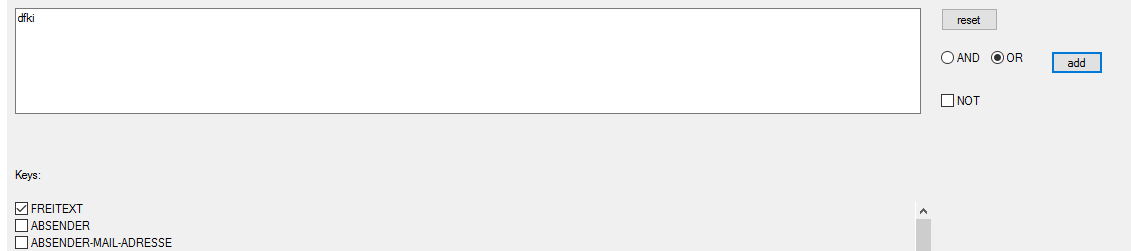
\includegraphics[width=1.1\textwidth]{images/b2}
	\caption{Keywords mit Freitext verkn�pfen (eigene Abbildung)}
	\label{b}
	
\end{figure}

\begin{figure} [http]
	
	\centering
	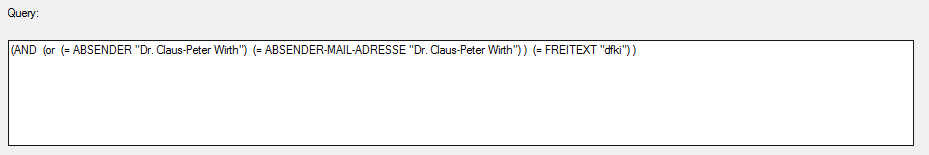
\includegraphics[width=1.1\textwidth]{images/b}
	\caption{Display (eigene Abbildung)}
	\label{c}
	
\end{figure}

\section{Ergebnis}
\begin{figure} [http]
	
	\centering
	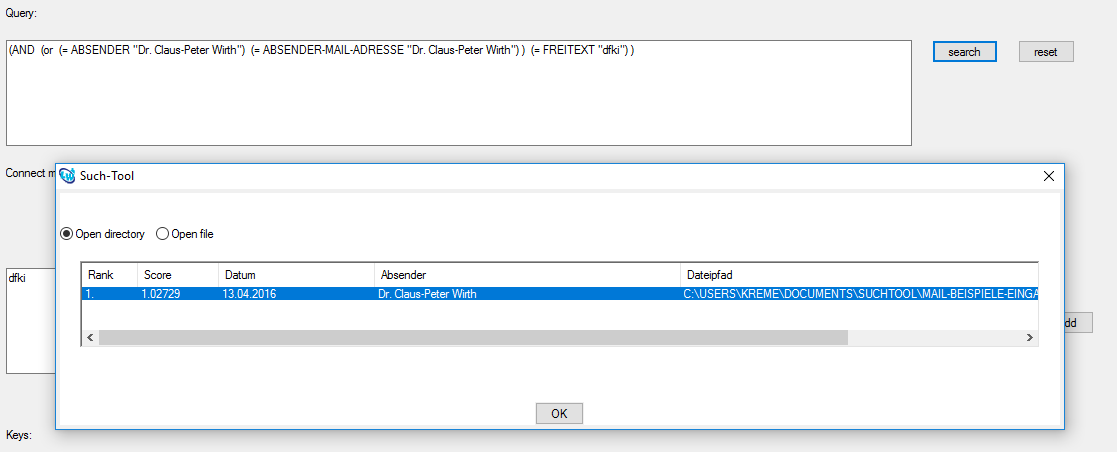
\includegraphics[width=1.1\textwidth]{images/c}
	\caption{Resultatfenster f�r obige Anfrage (eigene Abbildung)}
	\label{d}
	
\end{figure}

\begin{figure} [http]
	
	\centering
	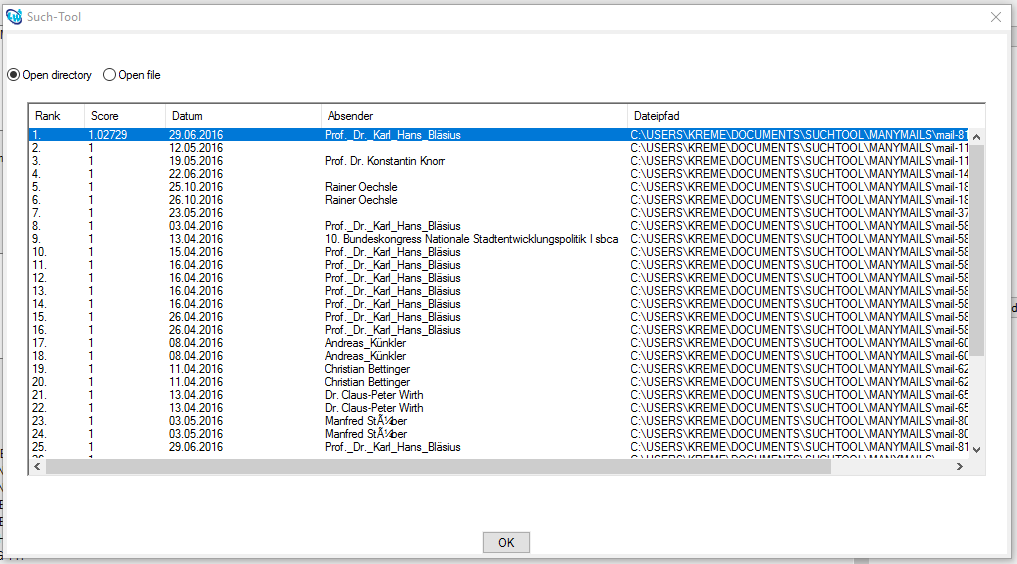
\includegraphics[width=1.1\textwidth]{images/results}
	\caption{Scrollbare Anzeige f�r viele Treffer (eigene Abbildung)}
	\label{res}
	
\end{figure}